\documentclass[12pt,a4paper]{article}

\usepackage[utf8]{inputenc}
\usepackage[indonesian]{babel}
\usepackage{graphicx}
\usepackage{geometry}
\usepackage{float}
\usepackage{listings}
\usepackage{xcolor}
\usepackage{array}
\usepackage{longtable}
\usepackage{amsmath}

\geometry{
    left=3cm,
    right=3cm,
    top=3cm,
    bottom=3cm
}

\lstset{
    basicstyle=\ttfamily\small,
    breaklines=true,
    frame=single,
    backgroundcolor=\color{gray!10},
    keywordstyle=\color{blue},
    commentstyle=\color{green!50!black},
    stringstyle=\color{red!60!black}
}

\begin{document}

\begin{titlepage}
    \centering
    {\Large \textbf{LAPORAN PROJECT BASED LEARNING}}\\[0.5cm]
    {\Large \textbf{ALGORITMA DAN PEMROGRAMAN}}\\[1cm]

    {\LARGE \textbf{Dashboard Monitoring Level Air Tandon Gedung Berbasis Rust}}\\[2cm]

    \textbf{Dosen Pengampu:}\\
    Ahmad Radhy, S.Si., M.Si.\\[1.5cm]

    \textbf{Disusun oleh:}\\[0.3cm]
    CRAFFTY HANA M.C. \hspace{0.5cm} 2042251054\\
    TIARA HEMAS E.P. \hspace{0.5cm} 2042251019\\[2cm]

    \textbf{Program Studi Teknik Instrumentasi}\\
    \textbf{Departemen Teknik Instrumentasi}\\
    \textbf{Institut Teknologi Sepuluh Nopember}\\[1cm]

    \textbf{2026}
\end{titlepage}

\tableofcontents
\newpage

\section{Pendahuluan}

Air merupakan kebutuhan penting dalam operasional gedung. Pada gedung bertingkat, air biasanya disimpan di dalam tandon sebelum didistribusikan ke berbagai bagian gedung. Level air pada tandon perlu dipantau agar tidak terlalu rendah maupun terlalu penuh.

Jika level air terlalu rendah, distribusi air dapat terganggu karena jumlah air di dalam tandon tidak mencukupi. Sebaliknya, jika level air terlalu tinggi, tandon dapat mengalami overflow atau luapan air. Oleh karena itu, diperlukan sistem monitoring level air yang mampu membaca level air, menentukan kondisi tandon, serta mengontrol pompa dan alarm secara otomatis.

Project ini dibuat dalam bentuk aplikasi terminal berbasis bahasa pemrograman Rust. Sistem ini mensimulasikan pembacaan level air tandon secara berulang, melakukan validasi data, kalibrasi sederhana, perhitungan sliding moving average 3 data terakhir, serta pengambilan keputusan untuk mengatur pompa dan alarm.

\section{Studi Kasus Instrumentasi}

Studi kasus yang digunakan pada project ini adalah sistem monitoring level air pada tandon gedung. Sensor yang digunakan disimulasikan sebagai sensor level air ultrasonik. Sensor memberikan data berupa persentase level air dari 0\% sampai 100\%.

Sistem akan menentukan status tandon berdasarkan hasil sliding moving average. Ketika level air rendah, pompa akan menyala. Ketika level air berada pada kondisi normal, pompa dan alarm akan mati. Ketika level air hampir penuh, sistem memberikan status hampir penuh. Ketika level air melebihi batas aman, sistem akan memberikan peringatan overflow dan menyalakan alarm.

\subsection{Aturan Status Level Air}

\begin{center}
\begin{tabular}{|c|c|c|c|}
\hline
\textbf{Level Air} & \textbf{Status} & \textbf{Pompa} & \textbf{Alarm} \\
\hline
0--20\% & Air Rendah & ON & OFF \\
\hline
21--80\% & Normal & OFF & OFF \\
\hline
81--95\% & Hampir Penuh & OFF & OFF \\
\hline
$>$95\% & Overflow Warning & OFF & ON \\
\hline
\end{tabular}
\end{center}

\section{Algoritma dan Flowchart}

\subsection{Algoritma Sistem}

Algoritma sistem monitoring level air tandon adalah sebagai berikut:

\begin{enumerate}
    \item Program dimulai.
    \item Sistem menginisialisasi objek \textit{Sensor}, \textit{Controller}, dan \textit{MonitoringSystem}.
    \item User memasukkan nilai level air dalam persen.
    \item Program memvalidasi data agar berada pada rentang 0 sampai 100 persen.
    \item Jika data tidak valid, program menampilkan pesan error dan meminta input berikutnya.
    \item Jika data valid, program melakukan kalibrasi sensor dengan menambahkan nilai offset.
    \item Data hasil kalibrasi disimpan ke dalam vector.
    \item Program menghitung sliding moving average dari 3 data terakhir.
    \item Program menentukan status tandon berdasarkan hasil sliding moving average.
    \item Program mengatur status pompa dan alarm.
    \item Program menampilkan dashboard monitoring.
    \item Program kembali meminta input level air berikutnya.
    \item Jika user mengetik \texttt{q}, \texttt{exit}, atau \texttt{stop}, program berhenti menerima input.
    \item Program menampilkan ringkasan akhir monitoring.
    \item Program selesai.
\end{enumerate}

\subsection{Flowchart Sistem}

Flowchart sistem monitoring level air tandon ditunjukkan pada Gambar \ref{fig:flowchart}.

\begin{figure}[H]
    \centering
    \includegraphics[width=0.85\textwidth]{../flowchart/flowchat_sistem.png}
    \caption{Flowchart Sistem Monitoring Level Air Tandon}
    \label{fig:flowchart}
\end{figure}

\section{Penjelasan Program Rust}

Program dibuat menggunakan bahasa pemrograman Rust. Program ini berbasis terminal dan dijalankan menggunakan perintah:

\begin{lstlisting}
cargo run
\end{lstlisting}

Program menerima input berupa nilai level air tandon dalam satuan persen secara berulang. Setiap data yang dimasukkan akan divalidasi agar berada pada rentang 0 sampai 100 persen. Data yang valid akan dikalibrasi, disimpan ke dalam vector, kemudian digunakan untuk menghitung sliding moving average dari 3 data terakhir.

Program akan terus menerima input sampai user mengetik \texttt{q}, \texttt{exit}, atau \texttt{stop}. Setelah program dihentikan, sistem akan menampilkan ringkasan akhir hasil monitoring.

Hasil sliding moving average digunakan sebagai dasar pengambilan keputusan untuk menentukan status tandon, mengatur pompa, dan mengatur alarm.

\subsection{Fitur Program}

Fitur utama program adalah sebagai berikut:

\begin{enumerate}
    \item Input level air tandon dalam persen secara berulang.
    \item Program berhenti ketika user mengetik \texttt{q}, \texttt{exit}, atau \texttt{stop}.
    \item Validasi input agar hanya menerima data 0 sampai 100 persen.
    \item Kalibrasi sensor sederhana menggunakan offset.
    \item Perhitungan sliding moving average dari 3 data terakhir.
    \item Penentuan status tandon secara otomatis.
    \item Kontrol pompa otomatis saat air rendah.
    \item Alarm overflow saat air melebihi batas aman.
    \item Visualisasi level air dalam bentuk bar terminal.
    \item Ringkasan akhir hasil monitoring.
\end{enumerate}

\section{Konsep OOP}

Rust tidak menggunakan konsep class seperti beberapa bahasa pemrograman lain. Namun, konsep pemrograman berbasis objek dapat diterapkan menggunakan \texttt{struct} dan \texttt{impl}. Pada project ini terdapat tiga objek utama, yaitu \texttt{Sensor}, \texttt{Controller}, dan \texttt{MonitoringSystem}.

\subsection{Struct Sensor}

Struct \texttt{Sensor} digunakan untuk merepresentasikan sensor level air. Struct ini memiliki atribut nama sensor, nilai pembacaan sensor, dan offset kalibrasi.

\begin{lstlisting}[language=Rust]
struct Sensor {
    name: String,
    value: f32,
    offset: f32,
}
\end{lstlisting}

Method utama pada \texttt{Sensor} adalah:

\begin{itemize}
    \item \texttt{new()} untuk membuat objek sensor baru.
    \item \texttt{read\_value()} untuk membaca nilai sensor.
    \item \texttt{calibrated\_value()} untuk menghitung nilai sensor setelah dikalibrasi.
\end{itemize}

\subsection{Struct Controller}

Struct \texttt{Controller} digunakan untuk mengatur status pompa dan alarm.

\begin{lstlisting}[language=Rust]
struct Controller {
    pump: bool,
    alarm: bool,
}
\end{lstlisting}

Controller memiliki method \texttt{control()} yang digunakan untuk menentukan status pompa dan alarm berdasarkan nilai sliding moving average. Jika level air rendah, pompa akan menyala. Jika level air melebihi 95\%, alarm akan menyala sebagai peringatan overflow.

\subsection{Struct MonitoringSystem}

Struct \texttt{MonitoringSystem} digunakan sebagai sistem utama yang menggabungkan sensor, controller, dan data hasil pembacaan sensor.

\begin{lstlisting}[language=Rust]
struct MonitoringSystem {
    sensor: Sensor,
    controller: Controller,
    data: Vec<f32>,
}
\end{lstlisting}

Vector \texttt{data} digunakan untuk menyimpan data level air yang telah dikalibrasi. Data tersebut kemudian digunakan untuk menghitung sliding moving average 3 data terakhir.

\section{Implementasi Komputasi Numerik}

Komputasi numerik yang digunakan pada project ini adalah \textbf{sliding moving average} dengan window 3 data terakhir. Metode ini digunakan untuk menghitung rata-rata dari maksimal tiga pembacaan sensor terbaru.

Sliding moving average digunakan agar pembacaan sensor lebih stabil terhadap noise, tetapi tetap responsif terhadap perubahan level air. Jika hanya menggunakan satu data terakhir, status sistem dapat berubah terlalu cepat akibat fluktuasi sesaat. Sebaliknya, jika menggunakan semua data sejak awal, data lama dapat terlalu memengaruhi hasil perhitungan.

Rumus sliding moving average adalah:

\[
SMA = \frac{\text{Jumlah data pada window}}{\text{Jumlah data dalam window}}
\]

Contoh data input:

\[
10, 50, 90, 98
\]

Dengan offset kalibrasi sebesar 1.0, data terkalibrasi menjadi:

\[
11, 51, 91, 99
\]

Karena window yang digunakan adalah 3 data terakhir, maka data yang dihitung adalah:

\[
51, 91, 99
\]

\[
SMA = \frac{51 + 91 + 99}{3} = 80.33
\]

Jadi nilai sliding moving average dari tiga data terakhir adalah 80.33\%.

\section{Kalibrasi Sensor}

Kalibrasi sensor dilakukan dengan menambahkan nilai offset pada nilai pembacaan sensor. Pada project ini digunakan offset sebesar 1.0.

Rumus kalibrasi:

\[
\text{Level Terkalibrasi} = \text{Level Aktual} + \text{Offset}
\]

Contoh:

\[
50 + 1 = 51
\]

Jadi jika level aktual adalah 50\%, maka level terkalibrasi menjadi 51\%.

\section{Hasil Pengujian}

Pengujian dilakukan dengan menjalankan program menggunakan input manual beberapa data level air secara berulang.

\subsection{Pengujian Input Manual Berulang}

Contoh input manual:

\begin{lstlisting}
Masukkan level air tandon:
10

Masukkan level air tandon:
50

Masukkan level air tandon:
90

Masukkan level air tandon:
98

Masukkan level air tandon:
q
\end{lstlisting}

Hasil kalibrasi:

\begin{center}
\begin{tabular}{|c|c|c|}
\hline
\textbf{Data} & \textbf{Level Aktual} & \textbf{Level Terkalibrasi} \\
\hline
1 & 10\% & 11\% \\
\hline
2 & 50\% & 51\% \\
\hline
3 & 90\% & 91\% \\
\hline
4 & 98\% & 99\% \\
\hline
\end{tabular}
\end{center}

Sliding moving average akhir:

\[
\frac{51 + 91 + 99}{3} = 80.33
\]

Status akhir sistem adalah hampir penuh, pompa OFF, dan alarm OFF.

\subsection{Pengujian Status Sistem}

Berikut adalah pengujian status sistem berdasarkan rentang level air:

\begin{center}
\begin{tabular}{|c|c|c|c|}
\hline
\textbf{Input Level} & \textbf{Level Terkalibrasi} & \textbf{Status} & \textbf{Output Kontrol} \\
\hline
10\% & 11\% & Air Rendah & Pompa ON, Alarm OFF \\
\hline
50\% & 51\% & Normal & Pompa OFF, Alarm OFF \\
\hline
90\% & 91\% & Hampir Penuh & Pompa OFF, Alarm OFF \\
\hline
98\% & 99\% & Overflow Warning & Pompa OFF, Alarm ON \\
\hline
\end{tabular}
\end{center}

\subsection{Pengujian Validasi Input}

Program juga diuji dengan input di luar rentang 0 sampai 100 persen. Jika user memasukkan nilai kurang dari 0 atau lebih dari 100, program akan menampilkan pesan error dan data tersebut tidak dimasukkan ke dalam perhitungan moving average.

Contoh input tidak valid:

\begin{lstlisting}
Masukkan level air tandon:
120

Error: level air harus berada pada rentang 0 sampai 100 persen.
\end{lstlisting}

\subsection{Screenshot Hasil Program}

Screenshot hasil program ditunjukkan pada Gambar \ref{fig:screenshot1} dan Gambar \ref{fig:screenshot2}.

\begin{figure}[H]
    \centering
    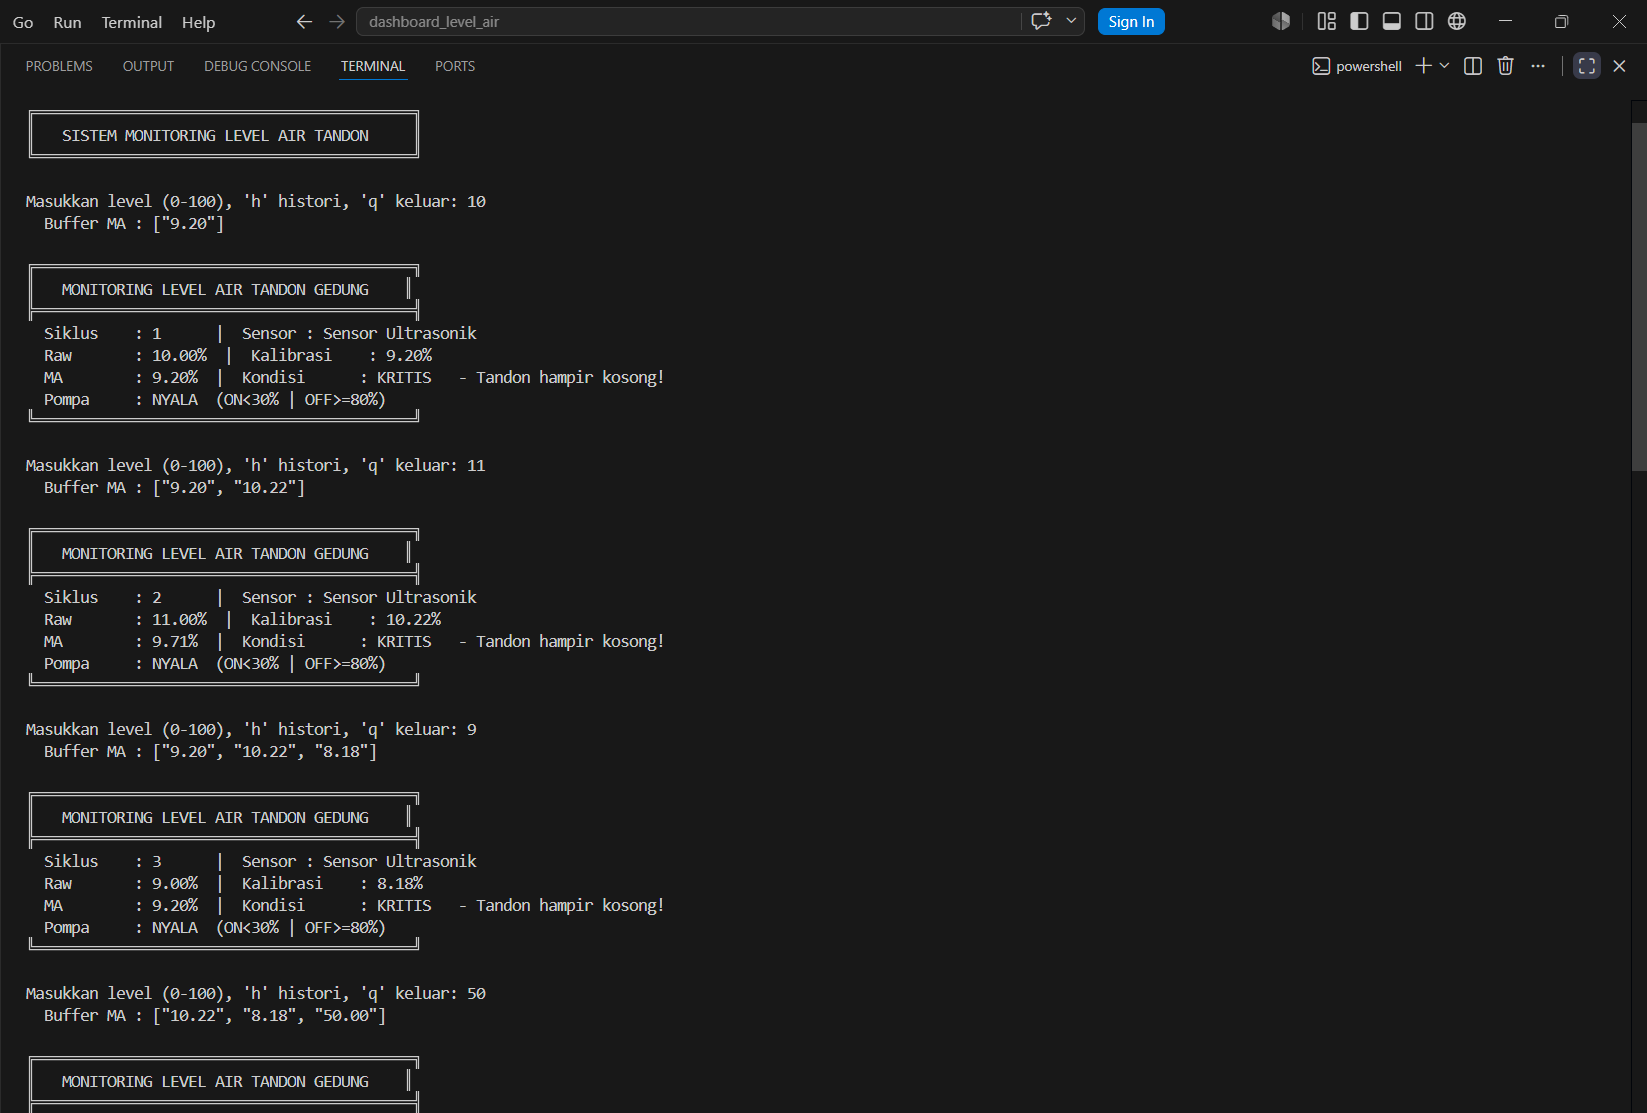
\includegraphics[width=0.85\textwidth]{../screenshot/hasil_program1.png}
    \caption{Screenshot Hasil Program 1}
    \label{fig:screenshot1}
\end{figure}

\begin{figure}[H]
    \centering
    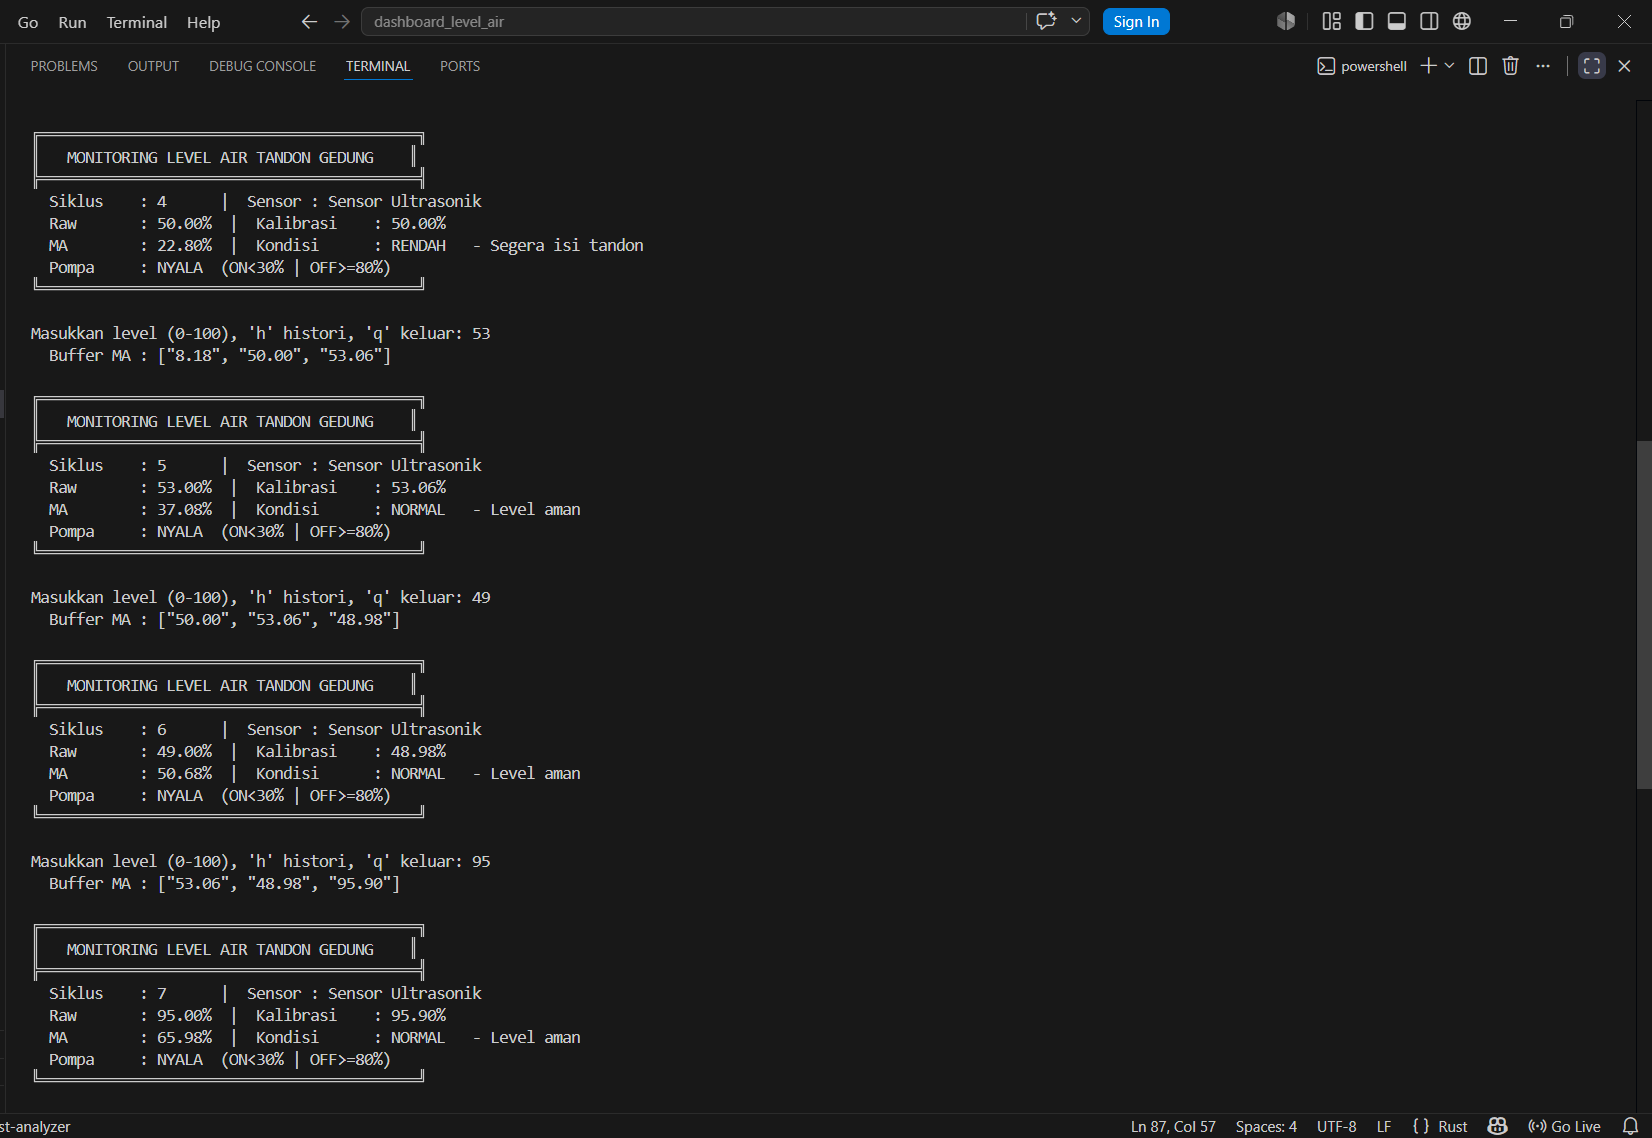
\includegraphics[width=0.85\textwidth]{../screenshot/hasil_program2.png}
    \caption{Screenshot Hasil Program 2}
    \label{fig:screenshot2}
\end{figure}

\section{Analisis Hasil}

Berdasarkan hasil pengujian, program dapat membaca input level air secara berulang, melakukan validasi, kalibrasi sensor, dan perhitungan sliding moving average 3 data terakhir. Program juga mampu menentukan status tandon berdasarkan rentang level air yang telah ditentukan.

Ketika moving average berada pada rentang 0--20\%, status sistem adalah air rendah dan pompa menyala. Ketika moving average berada pada rentang 21--80\%, status sistem adalah normal dan pompa mati. Ketika moving average berada pada rentang 81--95\%, sistem menunjukkan kondisi hampir penuh. Ketika moving average lebih dari 95\%, sistem memberikan peringatan overflow dan alarm menyala.

Penggunaan sliding moving average 3 data terakhir membuat sistem tidak hanya bergantung pada satu data sensor, tetapi mempertimbangkan beberapa data terbaru. Hal ini membuat hasil monitoring menjadi lebih stabil terhadap noise sensor, tetapi tetap responsif terhadap perubahan level air.

Validasi input juga berfungsi untuk memastikan data yang diproses berada pada rentang yang sesuai, yaitu 0 sampai 100 persen. Jika user memasukkan data di luar rentang tersebut, program akan menampilkan pesan error dan tidak memasukkan data tersebut ke dalam perhitungan.

Dengan sistem input berulang, program menjadi lebih menyerupai proses monitoring karena data dapat dimasukkan secara terus-menerus sampai user menghentikan program.

\section{Kesimpulan}

Project ini berhasil membuat aplikasi terminal berbasis Rust untuk monitoring level air tandon gedung. Program mampu membaca data level air secara berulang, melakukan validasi input, melakukan kalibrasi sederhana, menghitung sliding moving average 3 data terakhir, menentukan status tandon, serta mengontrol pompa dan alarm secara otomatis.

Konsep OOP berhasil diterapkan menggunakan \texttt{struct} dan \texttt{impl}, yaitu melalui objek \texttt{Sensor}, \texttt{Controller}, dan \texttt{MonitoringSystem}. Komputasi numerik berhasil diterapkan melalui metode sliding moving average dengan window 3 data terakhir.

Dengan adanya visualisasi level air dalam terminal dan sistem input berulang sampai user menghentikan program, aplikasi ini dapat digunakan sebagai simulasi sederhana sistem monitoring level air tandon gedung.

\end{document}